% !TEX root = ../Thesis.tex
\acresetall
\myChapter{Introduction}\label{ch:introduction}
\begin{flushright}{\slshape
		It's a magical world, Hobbes, ol' buddy\ldots\\
		\ldots Let's go exploring!}\\ \medskip
		--- Calvin\\Calvin and Hobbes, by\defcitealias{Watterson1996}{Bill Watterson}\citetalias{Watterson1996} \citep{Watterson1996}
\end{flushright}
\vspace{6cm}

Seeing and observing the object of interest has always been a crucial part of medical and biological research. If not by the naked eye, the object has been studied with ever-increasing resolution. In biomedical research, state of the art imaging methods include light and electron microscopy. Using advanced imaging methods like electron or x-ray microscopy, resolutions in the nanometer scale can be reached, which enables an extremely accurate rendition of the sample to be examined. Using three-dimensional methods like tomographic \ac{em} or especially \ac{srxtm} samples can be studied with a resolution in the nanometer~\cite{Downing2007} or sub-micrometer~\cite{Stampanoni2010} range.

\section{High resolution imaging}
One of the main problems with light and electron microscopy is the destructive sample preparation. For both methods, the sample has to be cut into physical sections with a thickness between 50--\SI{300}{\nano\meter}, generally around \SI{80}{\nano\meter}. This process destroys the three-dimensional structure of the sample and makes it very time consuming to reconstruct the three-dimensional placement of the sections to extract the structural information. \citet{Woodward2005} have shown that a three-dimensional reconstruction of parts of the gas exchanging region of the avian lung is feasible, but the process is both extremely time-consuming and needs very precise registration of the stack of sections which are cut from the sample.

An exception to this destructive sample preparation is offered by confocal microscopy~\cite{Minsky1961}. In confocal microscopy, light originating from outside the focal plane is excluded using a spatial pinhole. This enables the analysis of a sample section which is thicker than the optical focal plane of the objective. By positioning the focal plane stepwise through the volume of interest, the three-dimensional information of the sample can be obtained. This method obviously only works for samples with either a small enough thickness to still be translucent or for samples with a reasonably good penetration depth of the used light. The achievable volume of interest of confocal microscopy is thus limited and not sufficient for the analysis of the lung structure as presented in this work. 

In contrast to this, tomographic imaging makes it possible to non-destructively study the three-dimensional structure of a wide variety of samples, even opaque ones. Two-dimensional projections of the sample can be taken fairly easily using a multitude of electromagnetic radiation of different wavelengths (e.g.\ x-ray, infrared and visible light). These two-dimensional images contain the partial three-dimensional information of the sample volume which has been transversed by the radiation used to record the projection. If several projection images are acquired from different directions through the sample, the full three-dimensional information can be reconstructed using computed tomography~\cite{Hounsfield1976a}. \acf{srxtm} is a method to provide this three-dimensional information of millimeter sized samples in high resolution with voxel\graffito{A voxel or volumetric pixel is the \threed analogy to a \twod pixel.} sizes in the micrometer range~\cite{Bonse2008}. \ac{srxtm} was used as an underlying tool to obtain this information for all the samples presented in this thesis. The theory and concepts behind the tomographic reconstruction are explained in depth in~\autoref{ch:ct}.

\section{The mammalian lung}
Oxygen is an essential element for nearly every living multicellular organism\graffito{One exception being three newly discovered species of the animal phylum Loricifera which live inside permanently anoxic sediments~\cite{Danovaro2010}.}. The mammalian lung is the organ that transports this element into the body and provides the structure and function for the gas-exchange between the inhaled air in the alveolar space and the blood flowing in the capillaries in the lung tissue.

In the human body a tissue volume of approximately half a litre separates roughly the same amount of blood from an air volume of several litres~\cite{Weibel2009}, the lung is thus mostly built ``out of thin air''. The actual tissue portion of the lung is stretched up in the chest cavity and fills it with a delicate structure. The larger, purely conducting airways are built of multi-layer epithelial tissue and the finest parts, the alveolar septa are built of two thin cytoplasmic lamell\ae\ of the endothelial and type 1 epithelial cells separated by a single basement membrane; the average thickness of this tissue barrier is only about \SI{1.6}{\micro\meter} in the human lung\graffito{An overview of the development and the relevant structures of the lung is given in \autoref{ch:lung}.}~\cite{Weibel2009}.

The structure of the lung and the characteristics of the airways are vital for the function as an air conducting organ. Studying this structure makes it possible to gain important insights into both the development~\cite{Schittny2007a,Hyde2007} and function of the lung~\cite{Tsuda2002}. Three-dimensional imaging methods like \ac{ct} can give an insight into the structural relationships inside the lung, but cannot visualize the gas-exchange region of the lung through their limitation in resolution.

Tomographic imaging methods with higher resolutions like \ac{uct}~\cite{Hoffman2005} and \ac{srxtm}~\cite{Bayat2006,Bayat2009,Mund2008,Schittny2008,Tsuda2008} make it possible to extend the analysis deep into the lung, down to the gas-exchange region.

Certain structural parameters of the lung and especially of the terminal airway region as shown in \autoref{fig:alveoli} cannot be assessed using classical morphological methods based on histological sections of the lung tissue, since this slicing essentially destroys the three-dimensional structure of the lung. For example, extracting a three-dimensional view of multiple\graffito{With formidable effort, \citet{Woodward2005} managed to visualize components of the gas-exchange region of a duck.} functional units of the lung, the so-called acini and their interrelation is not possible only with the information from light or electron microscopy sections. But a study of their relations and structural changes is needed to characterize the changes the acini and lung structure undergo over the time-course of lung development. Using an imaging method like tomography that provides a full, unhindered and non-destructive view inside the lung makes it possible to reach this goal.

\renewcommand{\imsize}{\linewidth}%
\begin{figure}[htb]%
	\noindent\makebox[\textwidth]{%
		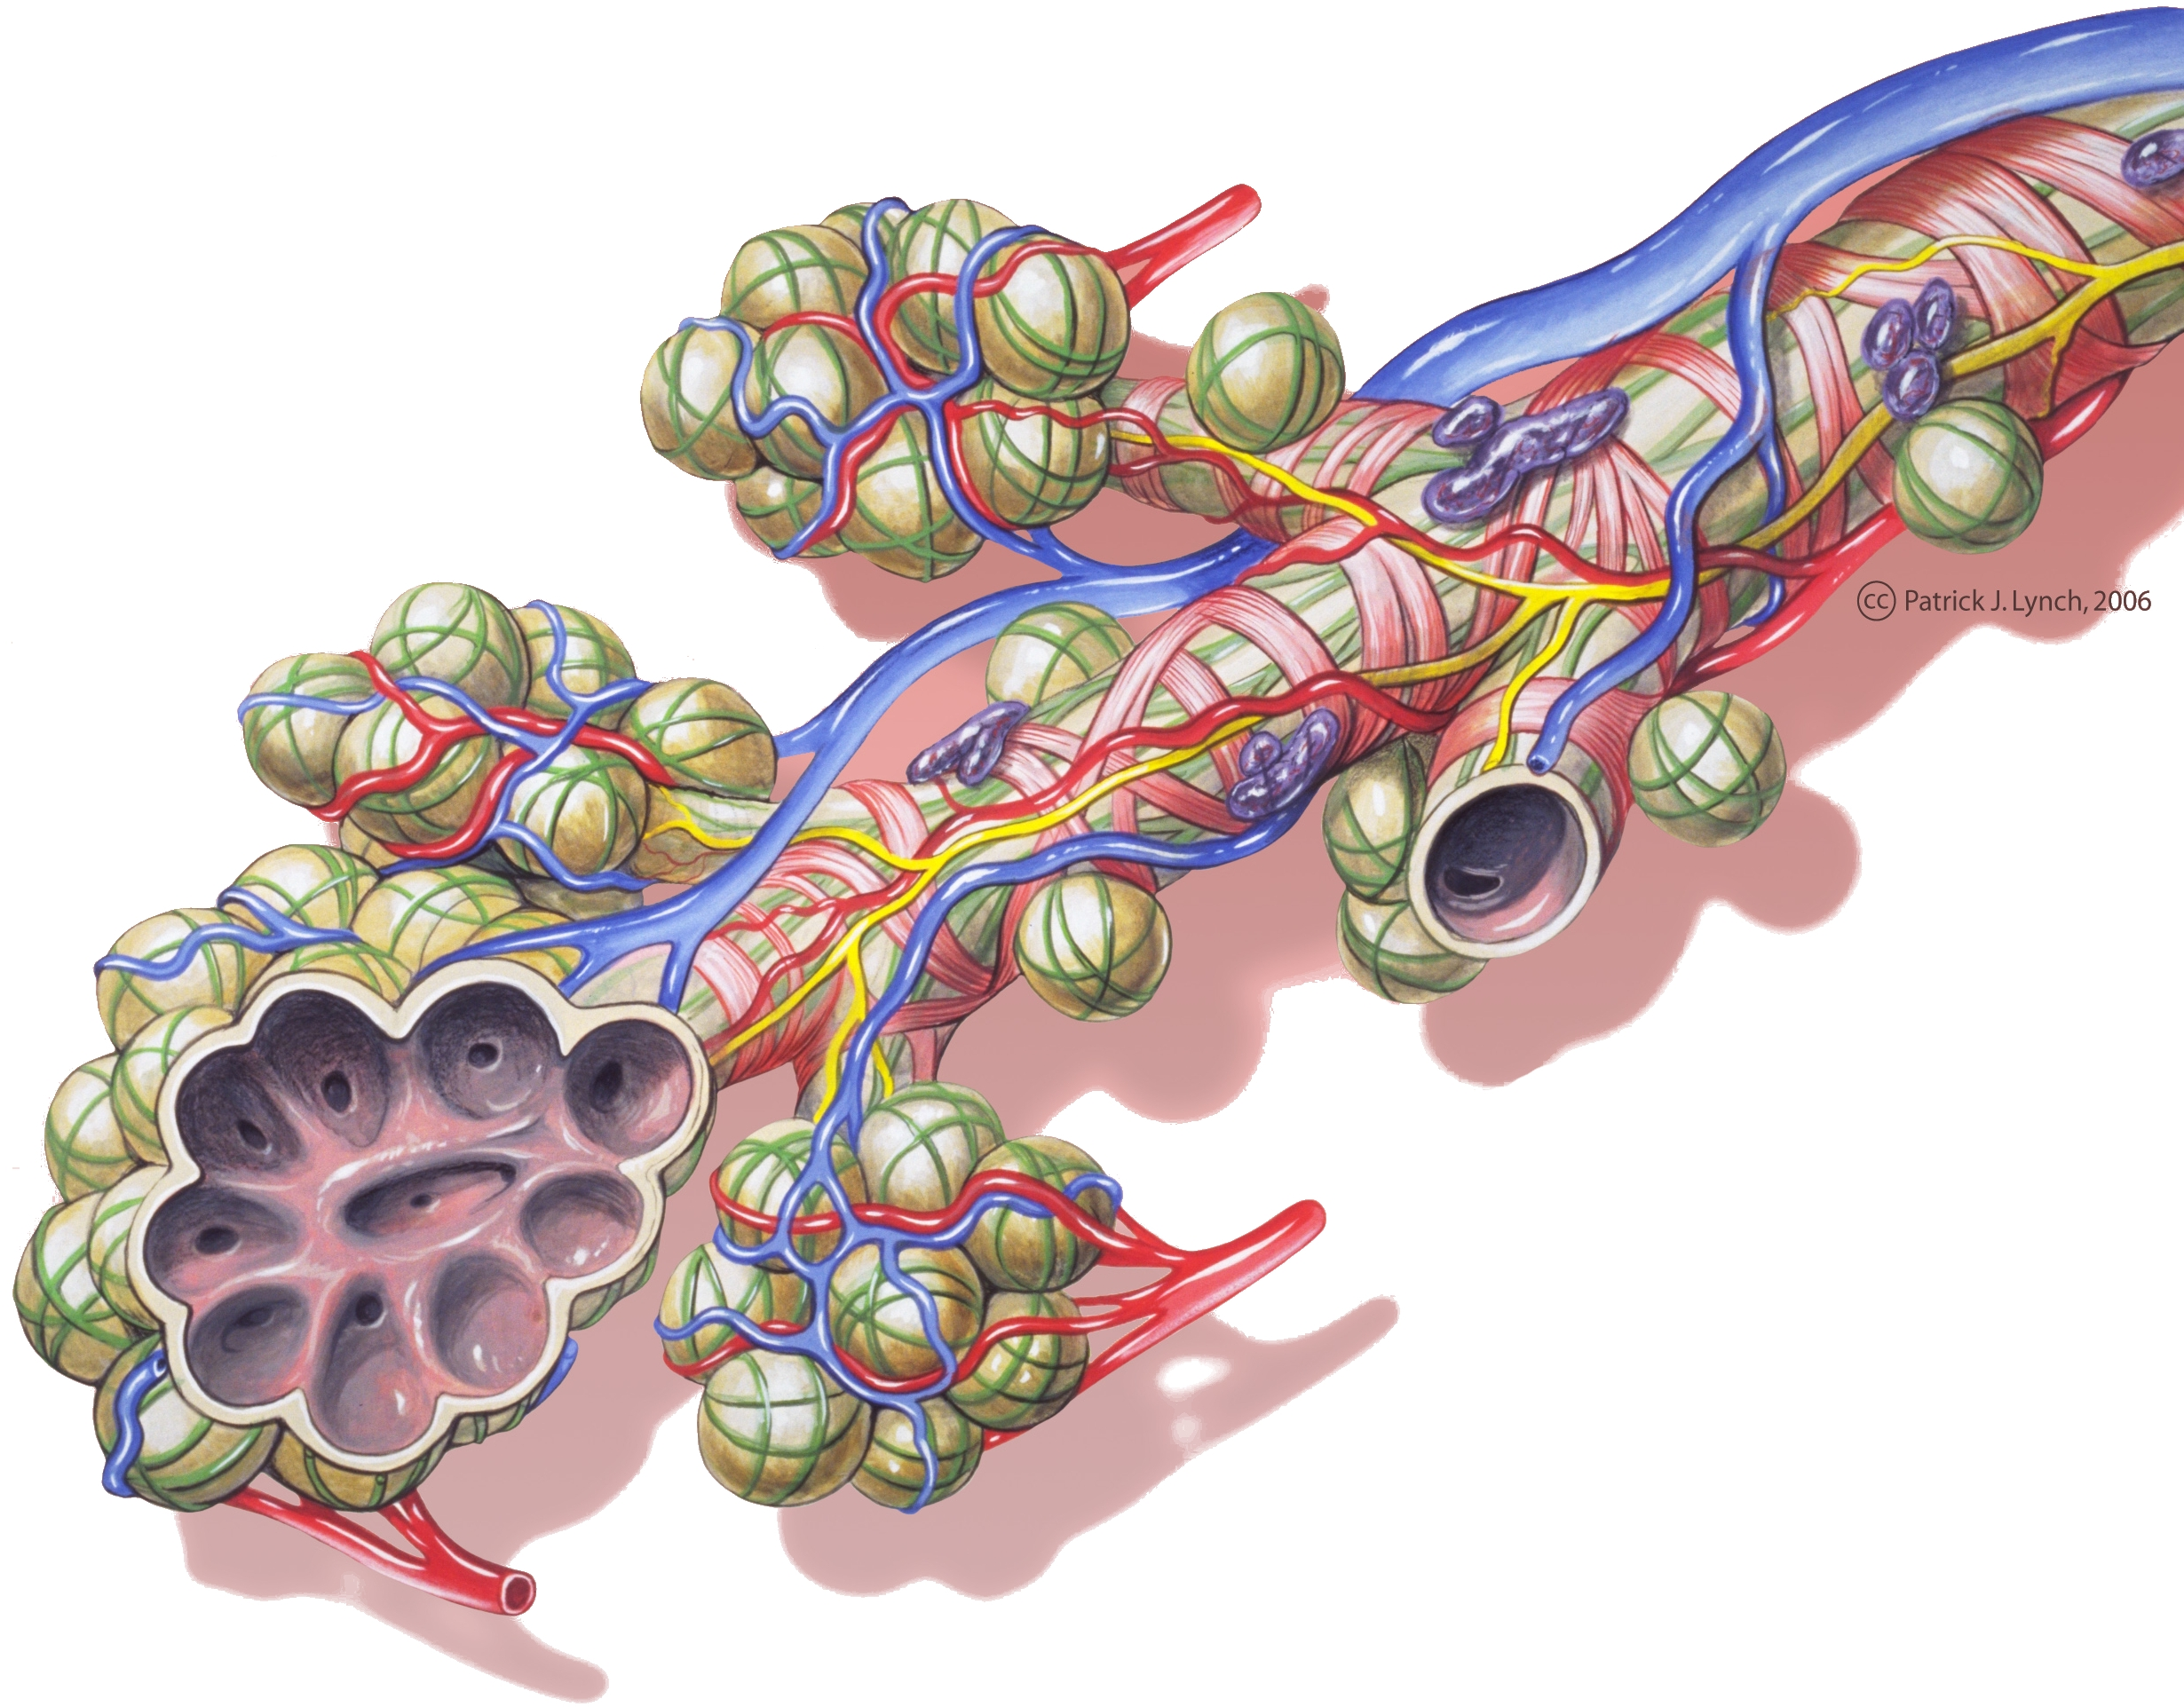
\includegraphics[width=\imsize]{img/Bronchial_anatomy_edit}%
	}%
	\caption[Bronchial anatomy detail]{Bronchial anatomy detail of alveoli and lung circulation. Adapted from~\cite{Alveoli}.}%
	\label{fig:alveoli}%
\end{figure}%

\section{Main goal of the Thesis}
From the beginning of my thesis at the Institute of Anatomy in September 2006 nearly everything I have worked on revolved around non-destructive tomographic imaging and detection of the finest structures in the mammalian lung, the so-called alveoli. 

The main focus of the work in our group lies on the study of the postnatal lung development, especially the changes in the airway structure~\cite{Burri1974}. As \citet{Weibel2009} described, the functional capacity of the lung as a gas exchange organ is determined by the fractal geometry, structure and peculiarities of the airways, almost opposite to the industrial design mantra \emph{\href{http://en.wikipedia.org/w/index.php?title=Form_follows_function&oldid=359712140}{Form follows function}}. Structural changes in the terminal airway ends like changes in alveolar number, increase in volume and changes in airway diameter~\cite{Burri1974} can be best studied using a fully three-dimensional imaging method like ultrahigh \todo{ultrahigh or ultra-high or ultra high?} resolution tomographic imaging. In close collaboration with the team of the beamline for \ac{tomcat} at the \ac{sls} we recorded a large number of tomographic scans of rat lung samples over the postnatal lung development up until postnatal day 60.

Modeling the structural parameters of the terminal airways using \ac{srxtm} data was one of the first goals achieved in this thesis. In a collaborative study I provided the three-dimensional reconstructions of multiple terminal airway regions inside several rat lung samples. Matching the structural parameters of the tomographic reconstructions to the same parameters previously assessed on two-dimensional histological sections from well characterized samples allowed an accurate reconstruction of the terminal airway ends in three dimensions. To our knowledge, the reconstructions of the alveolar and terminal airway region of rat lungs shown in \autoref{ch:tsuda2008} are the first ever published in a peer-reviewed publication. In a subsequent collaborative study, this data has been used for \ac{cfd} simulations of the airflow characteristics inside the alveoli, greatly increasing the fidelity of previous models of airflow deep in the lung~\cite{Tsuda2002}.

Another question approached during my thesis was focused on the interaction of particles in the lung parenchyma. To fully understand the influence of the terminal airway structure on the deposition sites of inhaled nanoparticles and sub-micron sized particles a three-dimensional visualization method based on tomographic data is needed, two-dimensional data is not sufficient for the full understanding of the interrelations of the terminal airway ends. Tomographic data is a perfectly suited tool for the three-dimensional structure of the terminal airways and localization of inhaled particles, but an exact analysis of the properties of such inhaled particles is not possible using \ac{srxtm} datasets. Since the particle size is in the order of the voxel size or resolution of the tomographic data around \SI{700}{nm}, additional imaging methods like \ac{em} are needed for a full analysis of the submicron particles in relation to the lung tissue. Using a multimodal approach combining three-dimensional high resolution \ac{srxtm} data and two-dimensional ultrahigh resolution two-dimensional \ac{em} data the interaction of particles deep in the lung and their exact localization in the airway tree has been studied; these results are presented in \autoref{ch:xrm2008}.

During the first experiments which focused on the changes of the structural parameters of the terminal airway over the course of the lung development the correct positioning of the lung samples in the field of view at the \ac{tomcat} beamline often relied on luck. This was because it is not possible to a judge or see the extent of single acini or connected airway segments inside a region of interest of 1.5$\times$1.5$\times$\SI{1.5}{\milli\meter} which corresponds to the field of view available at \ac{tomcat} prior to tomographic imaging.

More precisely, 
\begin{itemize}
	\item the acinus is bigger than the field of view at the magnification needed to resolve the finest structures in the lung, the tissue septa between the alveoli in the terminal airway ends and
	\item the acinus seems to be growing over time during lung development.
\end{itemize}

One goal of this thesis was to solve the problem stated in the first point. I developed a method to increase the field of view of tomographic endstations---especially \ac{tomcat}---while keeping the resolution of the resulting tomographic images on the level needed for the analysis of the finest structures in the lung. This goal has been reached with the implementation of a so-called \ac{wf-srxtm} scanning method at \ac{tomcat} has subsequently been published for the application at other tomographic endstations.

The second point mentioned\todo{Thesis oder thesis? $\rightarrow$ alles ersetzen!!!} above is the scope of ongoing research; analyzing the structure and size of the acini using a combination of segmentation and skeletonization\graffito{In image processing, the skeletonization of an arbitrary structure results in a thin version of said shape which is equidistant to the shape boundaries. The skeletonization process used in this thesis is described in \autoref{ch:discussion}.} of acini inside \ac{wf-srxtm} datasets already led to first promising results. The outlook in \autoref{ch:outlook} presents an overview of the achieved result and planned work.

\section{Outline of the Thesis}
This thesis is structured into the following parts:
\begin{itemize}
	\item [\autoref{part:introduction}] contains this introduction as a first chapter.
		
		\autoref{ch:lung} gives a short overview over the lung development.
	
		\autoref{ch:ct} explains the most important concepts in computed tomography and gives a short description of the \ac{tomcat} beamline, where all high resolution tomography experiments of this work have been performed.
	\item [\autoref{part:results}] contains publications written during the time of my Ph.D.\ Thesis at the Institute of Anatomy, which present the most exiting results achieved during my time at the \href{http://www.ana.unibe.ch/index_e.jsp}{Institute of Anatomy}.
	
		\autoref{ch:xrm2008} consists of a proceeding written for the 9\textsuperscript{th} \href{http://xrm2008.web.psi.ch/}{International Conference on X-Ray Microscopy} in Zürich, Switzerland, from the 21\textsuperscript{st} to the 25\textsuperscript{th} July 2008. This proceeding describes a method to precisely localize sub-micron sized gold particles in rat lungs through a combination of high resolution \acl{srxtm} and \acl{tem} and has been published in the Conference Series of the \href{http://iopscience.iop.org/1742-6596/}{Journal of Physics}.
		
		\autoref{ch:tsuda2008} consists of a paper published in the \href{http://jap.physiology.org/}{Journal of Applied Physiology} in which a novel image processing method for accurate three-dimensional reconstruction of the gas exchange region of the lung is presented. This method is based on a finite element analysis of datasets obtained with high resolution \acl{srxtm}.

		\autoref{ch:haberthuer2010} presents a method to increase the field of view of tomographic microscopy while keeping the advantage of a high resolution, something which is generally not possible. Additionally---through optimization of the acquisition protocol---the radiation dose inflicted on the sample can be greatly reduced. This paper has been accepted for publication in the \href{http://journals.iucr.org/s/}{Journal of Synchrotron Radiation}.

	\item [\autoref{part:discussion}] contains two chapters with a conclusive discussion of the obtained results and an outlook on further work.
	\item [\autoref{part:back matter}] finishes this thesis with a Curriculum Vit\ae, the Bibliography and the necessary documents for the \href{http://www.gcb.unibe.ch}{Graduate School for Cellular and Biomedical Sciences}.
\end{itemize}